\chapter{Implementation}
\graphicspath{{Chapter4/Figs/}{Chapter4/Figs/}}

This chapter goes into the implementation details of building the software-parts for the NIP of IDUN Technologies and the key events that occurred during the research and development such as the realisation of the novelty and need of a definition for a N/CI. Next to that the author also discusses other key aspects from building the system.

\section{Timeline}
\label{chapter4-timeline}

This is the implementation timeline as it was at the time of writing the thesis.

\begin{figure}[!ht]
  \centering
  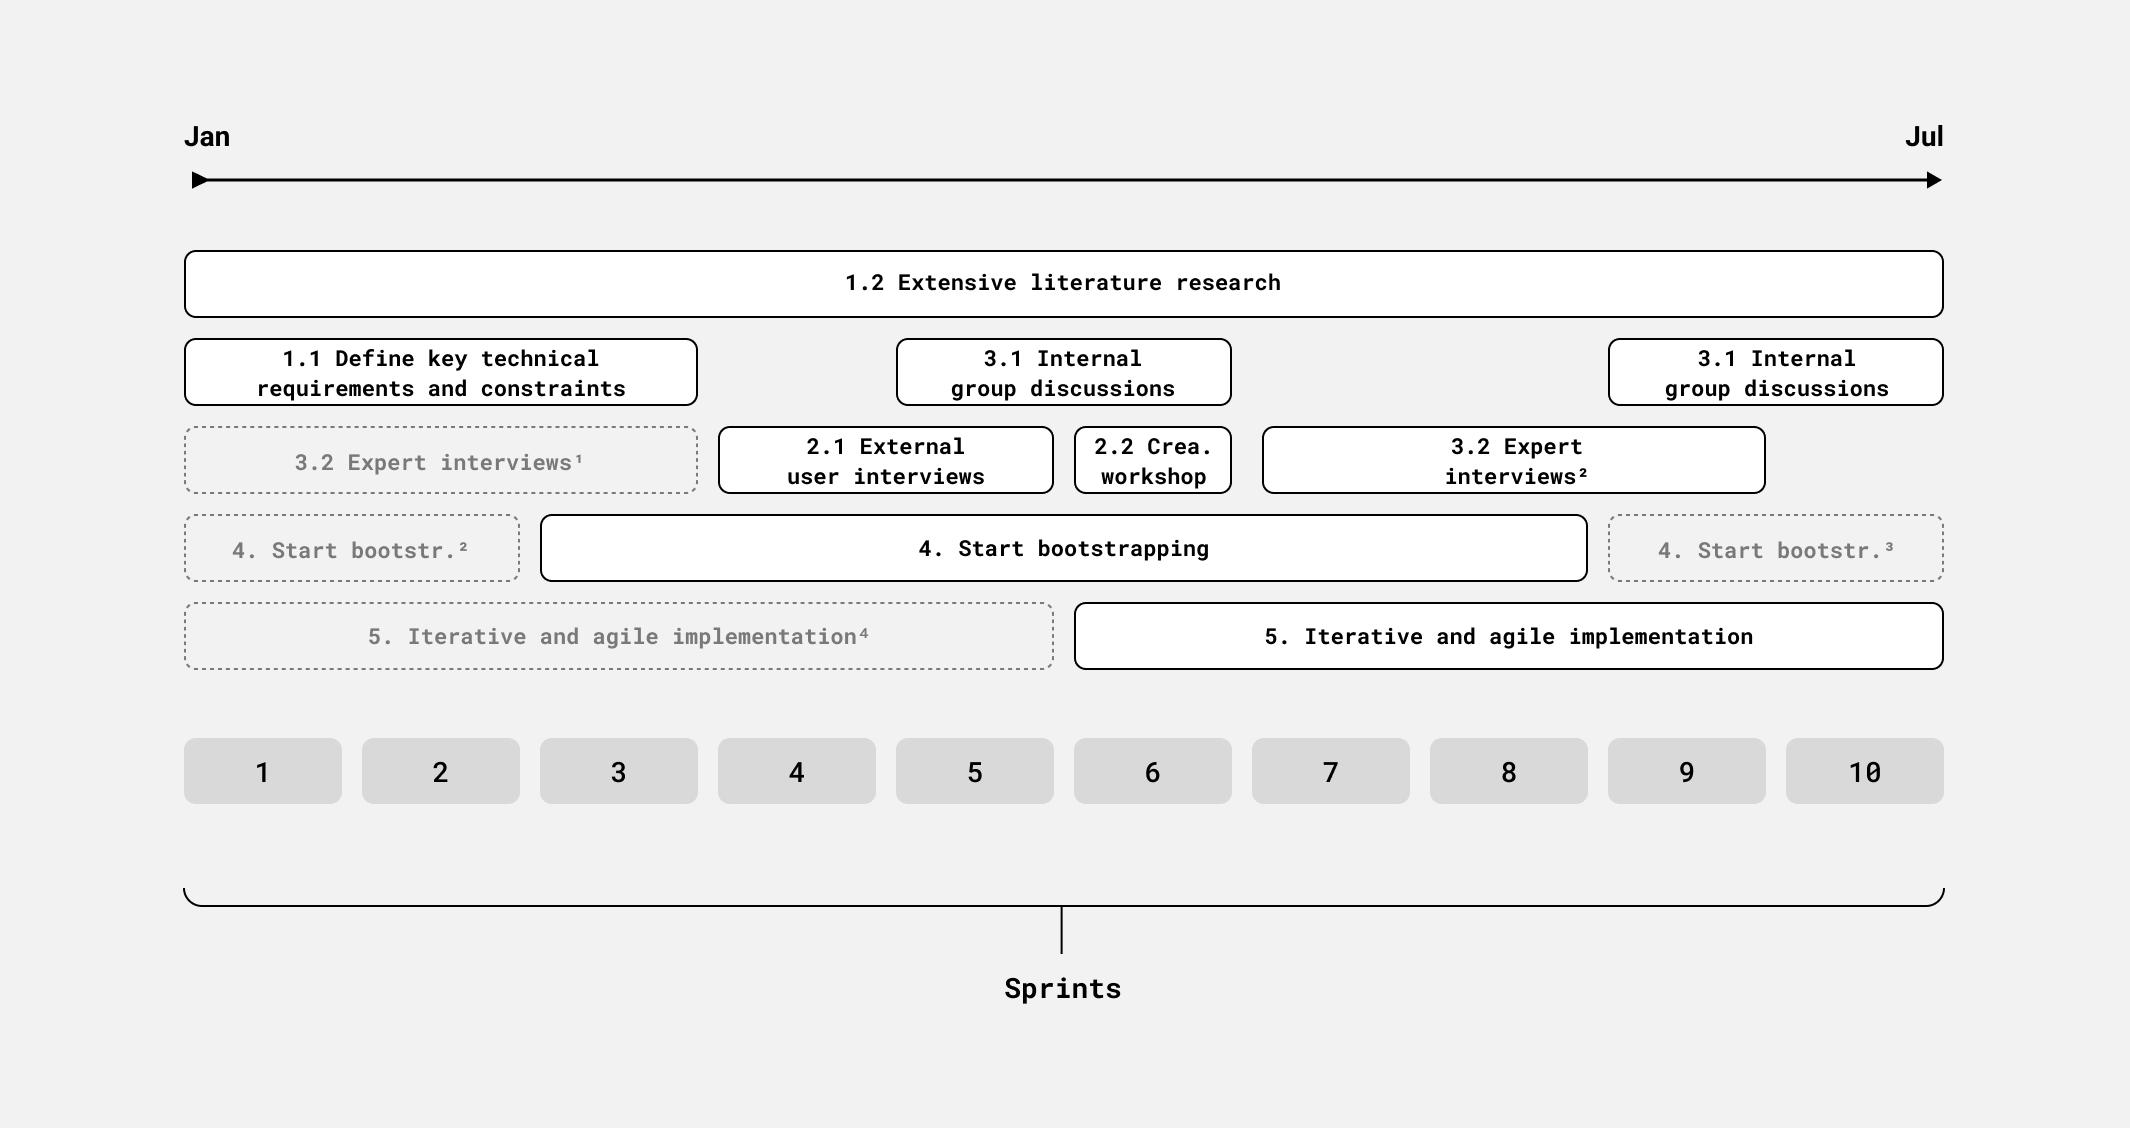
\includegraphics[width=\linewidth]{implementation-timeline.png}
  \caption{Timeline of the last 6 months.}
  \label{fig:implementation-timeline}
\end{figure}

Based on this we will go through each key event in a chronological manner, still starting with the most fundamental key events.

\begin{figure}[!ht]
  \centering
  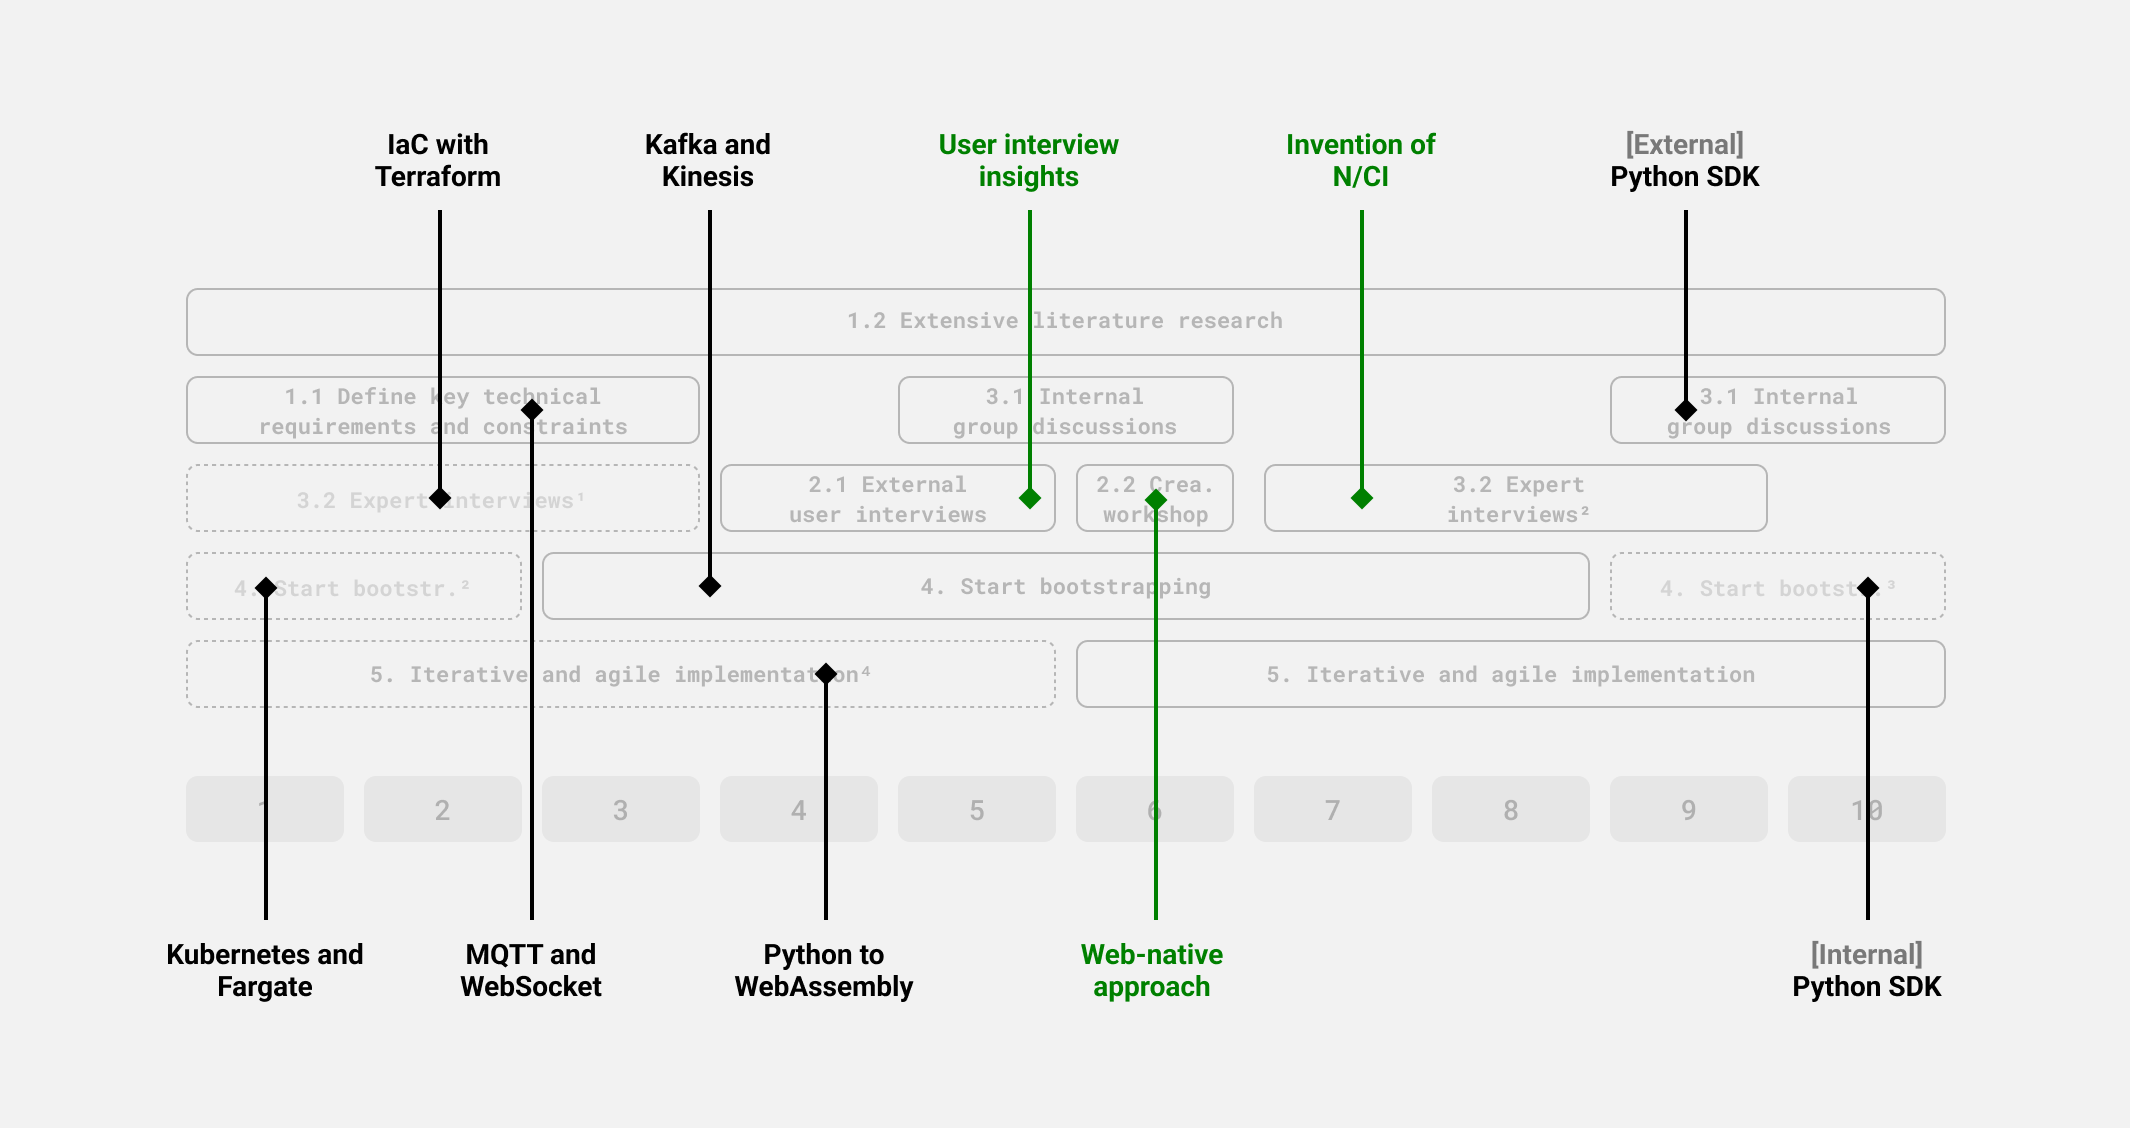
\includegraphics[width=\linewidth]{implementation-timeline-key-events.png}
  \caption{Key events on the previously showed timeline.}
  \label{fig:implementation-timeline-key-events}
\end{figure}

% empirical software engineering done in the case study based on user-centred design process via user interviews or expert interviews and internal group discussions and ongoing literature research.
% MENTION analysis paralysis

\section{Key events}
\label{chapter4-key-events}
% TODO create timeline in Figma

\subsection{User interview insights}
\label{chapter4-user-interview-insights}
% show image of mark and the author doing the user interview

\subsection{Invention of N/CI}
\label{chapter4-invention-of-nci}
% make the connection why the author talked about it in the beginning already

\subsection{Python to WebAssembly}
\label{chapter4-python-to-webassembly}
% mention sprint that we committed to that one

\subsection{Kubernetes and Fargate}
\label{chapter4-kubernetes-and-aws-fargate}
% quickly explain why microservices
% mention workshop with nuvibit (expert interview)
% mention centralised system rather than distributed

\subsection{Kafka and Kinesis}
\label{chapter4-kafka-aws-kinesis}
% mention workshop with nuvibit (expert interview)

\subsection{IaC with Terraform}
\label{chapter4-iac-with-terraform}
% mention workshop with nuvibit (expert interview)
% mention workshop with sascha from piavita

\subsection{MQTT and WebSocket}
\label{chapter4-mqtt-and-websocket}
% show image of andy on the whiteboard

\subsection{Web-first approach}
\label{chapter4-web-first-approach}
% mention dog feeding and vercel

\subsection{Python SDK}
\label{chapter4-python-sdk}
% mention internal discussions with michel (group discussion)
% mention github limitation of private pypi and registry in general
% mention again the no focus on GUI part from before

\section{Key aspects}
\label{chapter4-key-aspects}

\subsection{Stream-based events}
\label{chapter4-stream-based-events}
% explain event based architecture and the paradigm-shift in building stream based architectures

\subsection{Critical and non-critical}
\label{chapter4-critical-and-non-critical}
% mention the concept from the book and batch processing

\subsection{Hardware-accelerated encryption}
\label{chapter4-hardware-accelerated-encryption}
% mention server-side rendering for privacy
% mention discussion with Andy

\subsection{Per-device auth and opt-in}
\label{chapter4-user-side-opt-in}
% show opt-in wireframes

\subsection{Graph database}
\label{chapter4-graph-database}

\subsection{Feature store and MLOps}
\label{chapter4-feature-store-and-mlops}
% explain MLOps and outlook with Kubeflow
% mention data lakes and data warehouse
% mention internal SDK for feature extraction and experiments
% what is feature extraction and the process
% show image from Wadda

    % However, in practice, it appears that simply making data available quickly—even if it is in a quirky, difficult-to-use, raw format—is often more valuable than trying to decide on the ideal data model up front [54].
